\documentclass[../report.tex]{subfiles}
\begin{document}
\graphicspath{{img/}{../img/}}

The architecture of the DAL (See figure \ref{fig:DALclassdiagram}) has been implemented to support NFR-07 and NFR-08, which state that it must be possible to add support for new types of media and to add new functionality. The DAL is abstracting concrete implementation from the Business Logic Layer through a bridge pattern. This has been done so that persistence modules can be swapped without changes in the layer above, if the persistence needs to be updated or changed to another technology. The DAL is using the object-mapper pattern. This means that the storage layer does not know anything about the object model. This is done so that if a new entity were to be added, only the object model has to been updated in order to implement the change. 

A relational database management module has been implemented using Entity Framework (EF). EF is a good choice as it supports easy access to the database. The performance of EF is not as good as hard coded SQL-queries, but it is much more flexible and dynamic. The EF module is using the transaction state pattern to ensure that the database is consistent. The state pattern keeps track of the states of the entities, and only when Save Changes is invoked, the data is actually saved to the persistent module. This ensures that if the program were to crash while working on ongoing transactions, the persistent data integrity would not be violated. To improve performance while using the EF the database uses foreign keys which the EF uses for making property references for easy mapping between objects.

\begin{figure}[H]
\centering
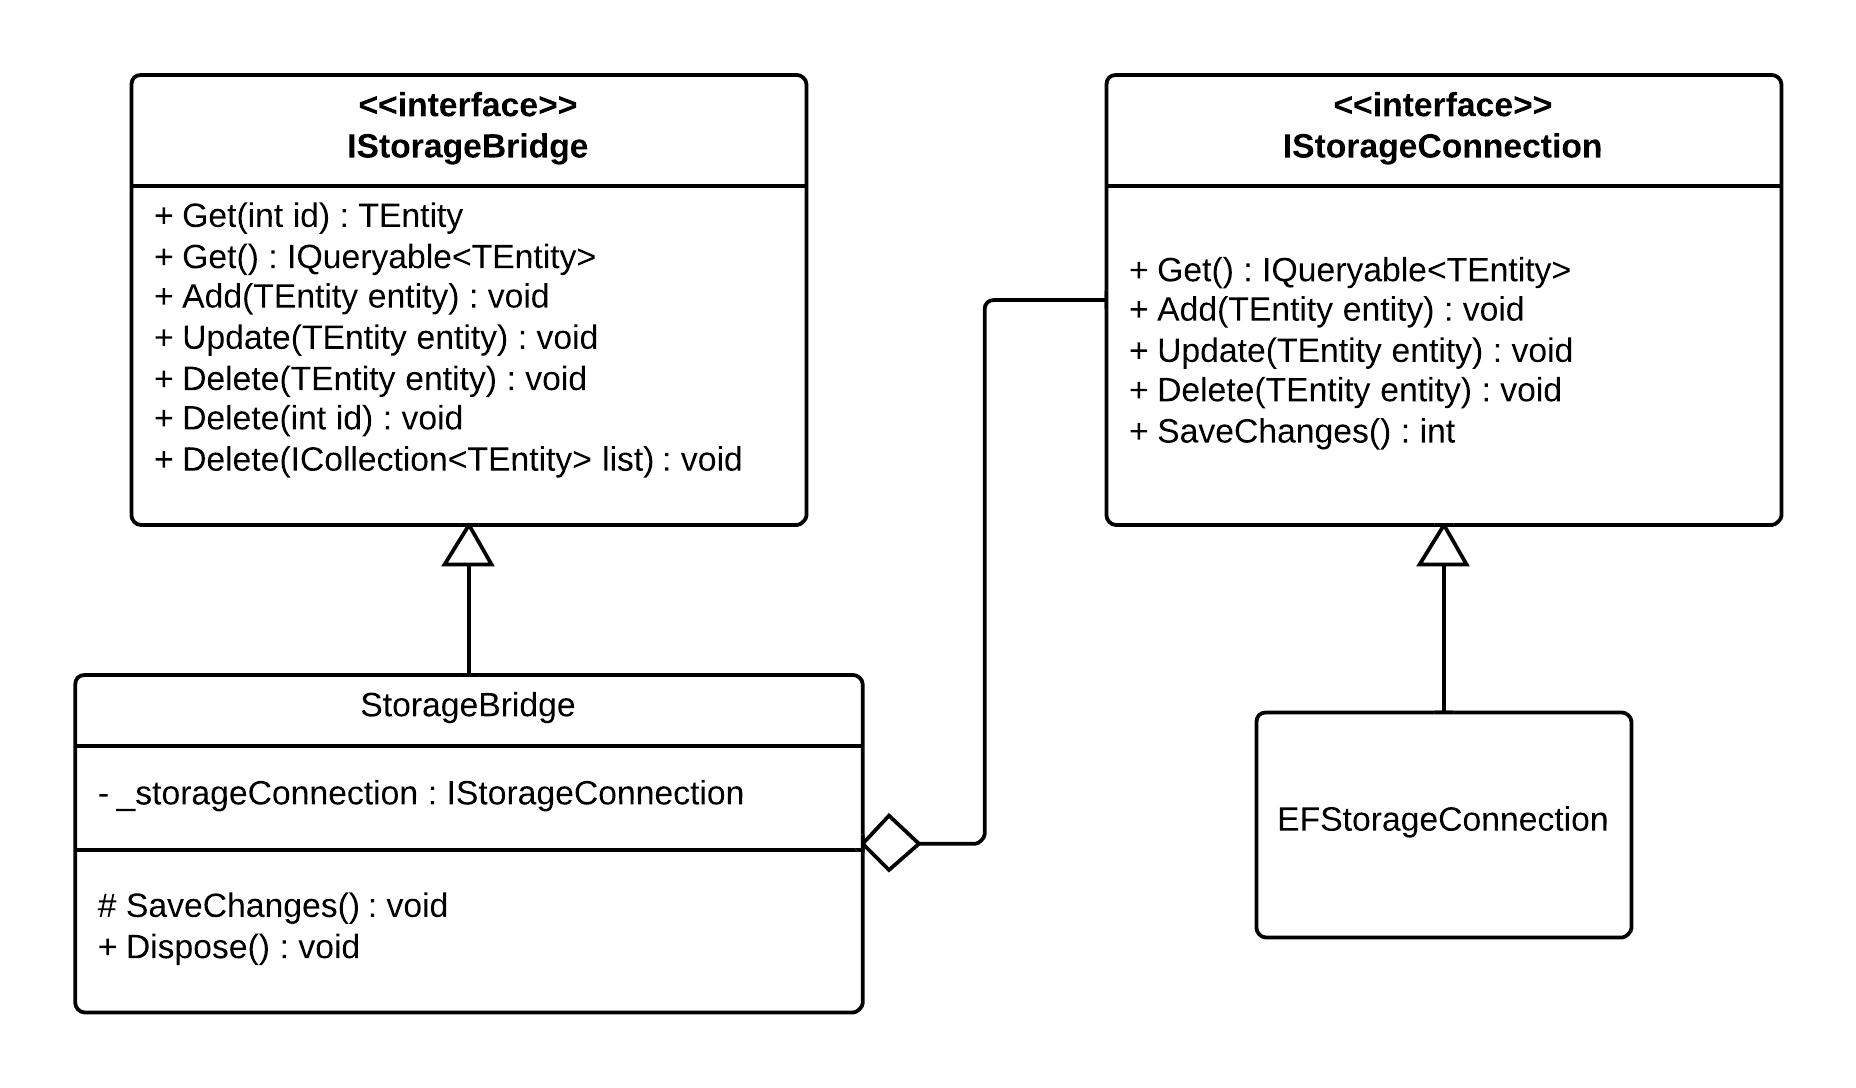
\includegraphics[width=\linewidth]{DALclassdiagram.png}
\caption{Data Access Layer architecture}
\label{fig:DALclassdiagram}
\end{figure} 

\end{document}